\part{Desenvolvimento}
\chapter{Desenvolvimento}

\section{Desenvolvimento da Visão Geral da Plataforma em TypeScript}
\section{Apresentação da estrutura, funcionalidades e interface planejadas para a plataforma.}
\section{Escolhas tecnológicas e considerações de usabilidade}
\subsection{A implementação da autenticação OAuth 2.0}
O OAuth 2.0 é o protocolo central que representa um pilar sólido de segurança e o gerenciamento eficaz dos acessos às sessões de TCI na plataforma. Este protocolo de autorização é fundamental para o processo, permitindo que a plataforma obtenha acesso limitado a contas de usuários em serviços HTTP sem a necessidade de enviar diretamente usuário e senha. Em essência, o usuário delega a um determinado aplicativo acesso aos seus dados em um serviço ou API específicos.\cite{OAUTH}Ao adotar o OAuth 2.0 do Google neste projeto, não apenas garante um método confiável para autenticar usuários, mas também preserva a integridade dos dados, permitindo que somente usuários autorizados tenham acesso à plataforma. Essa escolha tecnológica não só oferece solidez ao processo de autenticação, mas também acrescenta uma camada adicional de segurança ao ambiente da plataforma.

No contexto do fluxo de autenticação, desde o redirecionamento do navegador até a obtenção e validação do token de acesso, há uma atenção especial às considerações de usabilidade. Durante o processo de login, a plataforma direciona o navegador para um URL do Google, incorporando parâmetros que indicam o tipo de acesso desejado. Nesse momento, o usuário realiza o login com a Conta do Google, seleciona a sessão e, crucialmente, concede as permissões necessárias. Após o login, o usuário é solicitado a confirmar se deseja conceder as permissões requisitadas pela plataforma. A inclusão desses elementos visa não apenas garantir a segurança, mas também oferecer uma experiência de usuário intuitiva e transparente. Abaixo uma imagem exemplificando o fluxo de autenticação realizado pelo OAuth 2.0 do Google\cite{OAUTHACESS}:

\begin{figure}[!h] % ambiente usado para inserção de imagens
    \centering
    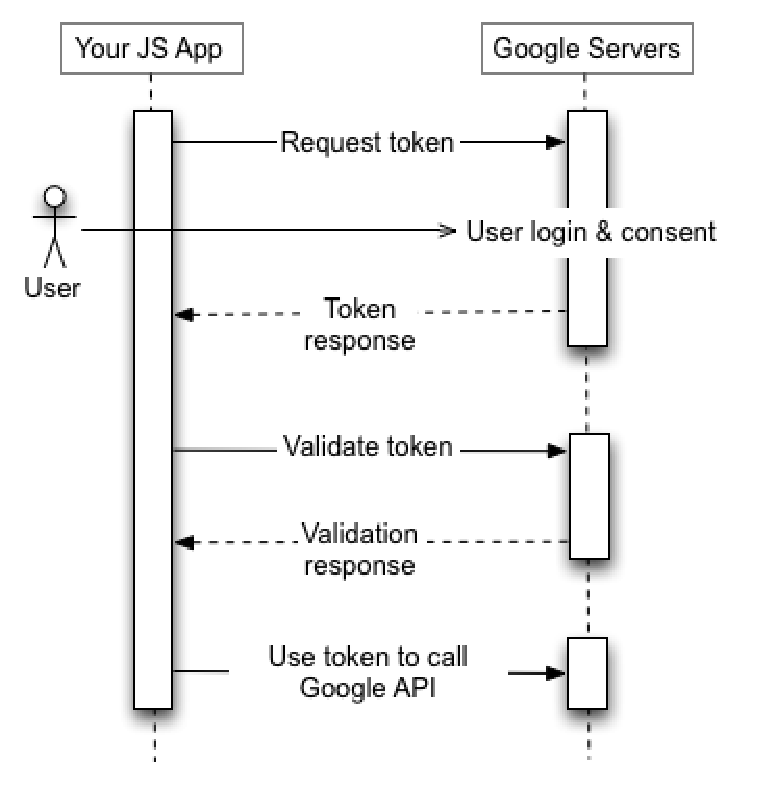
\includegraphics[scale=0.5]{latex/figuras/oauth.pdf}
    \caption[A implementação da autenticação OAuth 2.0]
    {Fluxo de autenticação realizado pelo OAuth 2.0 do Google}
\end{figure}

\pagebreak Além disso, a abordagem dos escopos provenientes do protocolo OAuth 2.0 do Google destaca-se como um componente crucial da estratégia de permissões. A inclusão desses escopos na resposta do token desempenha um papel vital para acessar recursos específicos do projeto, alinhando as escolhas tecnológicas com a usabilidade da plataforma. Dessa forma, os usuários fornecem apenas o essencial para o acesso aos recursos e funcionalidades pertencentes ao projeto, contribuindo para uma experiência mais personalizada e segura. A seguir, apresenta-se a relação de escopos provenientes do protocolo OAuth 2.0 do Google, os quais foram empregados no desenvolvimento da plataforma \cite{OAUTHSCOPES}:

\item \textit{\textbf{openid}} → Associação do usuário às suas informações pessoais presentes no Google;
\item \textit{\textbf{userinfo.email}} → Visualização do endereço de e-mail principal associado à Conta do Google;
\item \textit{\textbf{userinfo.profile}} → Acesso e visualização de informações pessoais, incluindo aquelas disponibilizadas publicamente;
\item \textit{\textbf{calendar}} → Permissão para gerenciar todas as agendas às quais o usuário tem acesso por meio do Google Calendar.

Os tokens de acesso são válidos somente para o conjunto de operações e recursos descritos no escopo. Por exemplo, está sendo usado na plataforma um token de acesso emitido para a API Google Calendar, ele não concederá acesso à uma API Google Contacts. O aplicativo precisa armazenar o token de atualização para uso futuro e usar o token de acesso para acessar uma API do Google. Quando o token de acesso expira, o aplicativo usa o token de atualização para conseguir um novo.

Para complementar, a política de expiração definida para os tokens foi um tempo de 24 horas para o token de atualização e um tempo mais curto, 30 minutos, para o token de acesso, evidenciando uma consideração equilibrada de usabilidade e segurança. Essa abordagem visa não apenas a proteção contra acessos não autorizados, mas também a otimização da experiência do usuário, evitando logins frequentes.

Assim, as escolhas tecnológicas incorporadas na implementação do OAuth 2.0 refletem uma busca constante por segurança robusta, ao mesmo tempo em que priorizam uma experiência do usuário coesa e eficiente na plataforma.


\chapter{Integração da Psicologia na Visão Geral da Plataforma}
A integração da Psicologia na Visão Geral da Plataforma ocorre através do uso intercambiável da psicoterapia online e da Psicoterapia baseada na internet. Isso traz benefícios que tornam a Terapia Comunitária Integrativa (TCI) mais acessível a um público mais amplo, superando barreiras geográficas. Na psicoterapia online, as pessoas podem participar de grupos terapêuticos remotamente, independentemente de sua localização física, o que facilita a participação de pessoas com diferentes origens e culturas.

A plataforma oferece flexibilidade de horários tanto para terapeutas quanto para participantes, facilitando a adesão aos grupos terapêuticos comunitários integrativos. Além disso, permite a criação de comunidades virtuais que se estendem além das sessões de terapia, possibilitando conexões entre os participantes, compartilhamento de recursos e apoio mútuo, fortalecendo os laços comunitários.

A Psicoterapia baseada na internet é incorporada à plataforma por meio de uma página com recursos multimídia, enriquecendo as experiências terapêuticas com vídeos que promovem uma sensação de bem-estar. Isso contribui para a diversidade e inclusão nos grupos terapêuticos, proporcionando uma compreensão mais abrangente dos benefícios dessa abordagem.

A proposta de criar links automatizados do Google Meet para as Rodas de Terapia Comunitária Integrativa (TCI) facilita o gerenciamento das sessões pelos terapeutas. Eles podem pré-determinar datas e horários, sincronizando automaticamente com o Google Calendar. Isso otimiza o tempo do terapeuta, permitindo que se dedique a outras atividades enriquecedoras.

Para os alunos interessados, a proposta oferece uma organização clara dos horários e datas das rodas de TCI, proporcionando autonomia na escolha das sessões terapêuticas que mais se adequam às suas rotinas universitárias.

A abordagem da Terapia Comunitária Integrativa (TCI) promove um enfoque intercultural que celebra a diversidade cultural. Reconhecendo a relação intrínseca entre desenvolvimento humano e contextos culturais, a TCI destaca o papel adaptativo do facilitador para garantir a qualidade das interações em grupo, mesmo em um ambiente online.

Para a realização das sessões online, a plataforma oferece uma experiência aprimorada, permitindo reunir pessoas para as rodas de psicoterapia comunitária integrativa por meio da tecnologia. O uso do Google Meet facilita a interação, criando um espaço virtual acolhedor onde os participantes podem compartilhar suas histórias e momentos, sem julgamentos.

A possibilidade de compartilhar recursos multimídia, por meio de uma playlist de vídeos no YouTube conectada à plataforma, enriquece a experiência terapêutica. Essa tecnologia apoia visualmente o processo terapêutico, proporcionando bem-estar e valorização cultural em momentos além das sessões de terapia.

Esses elementos, entrelaçados por representações que geram identificações, formam a base para um processo de cura significativo, potencializando mudanças individuais e comunitárias. A plataforma promove a compreensão e integração ativa das diversas dimensões culturais, valorizando a diversidade como essencial para o bem-estar emocional e social da comunidade.

Os avanços na tecnologia e na comunicação têm permitido a inclusão de recursos que favorecem a manutenção da saúde mental. É importante ressaltar que a concepção de saúde é profundamente influenciada pela cultura, e a TCI reconhece e respeita essas diversas visões de mundo.

Além disso, a Terapia Comunitária Integrativa defende a sintonia do indivíduo com as emoções e sentimentos despertados pelo contato, exigindo uma elevada auto-percepção. Incentiva a disposição para ouvir e compreender o outro, abrindo espaço para novas perspectivas e ressignificações daquilo que anteriormente era considerado imutável ou insuperável. Isso promove um ambiente propício ao crescimento pessoal e à construção de relações mais saudáveis, consolidando a visão integral da plataforma como um facilitador de bem-estar emocional e social.


\chapter{Engenharia Eletrônica na Implementação da Plataforma}
\section{Exploração das contribuições específicas da Engenharia Eletrônica no desenvolvimento da plataforma.}
\section{Destaque de tecnologias e recursos eletrônicos que podem ser aplicados.}

\chapter{Considerações Éticas e Privacidade de Dados}

Nos últimos anos, as inovações tecnológicas têm desempenhado um papel crucial na evolução dos serviços de saúde mental. A crescente demanda por atenção à saúde mental, aliada às possibilidades oferecidas pela tecnologia, resultou no desenvolvimento de novas modalidades de atendimento psicológico. O Conselho Federal de Psicologia (CFP), reconhecendo a importância desse avanço, regulamentou o atendimento psicoterápico remoto como uma prática profissional permitida e readequou a resolução para atender o contexto mundial atual.

Os atendimentos psicológicos online têm se destacado pela atratividade técnica, ampliando o alcance dos serviços de atenção à saúde mental. Essa modalidade adapta o cuidado sem necessidade de contato presencial, garantindo resultados efetivos e observando os aspectos éticos e legais da psicologia.\cite{SIEGMUND} A Terapia Comunitária Integrativa (TCI), reconhecida pelo Ministério da Saúde como uma abordagem psicossocial avançada, também abraçou a era digital. O Polo Formador em TCI Afinando Vidas, diante dos desafios impostos pela pandemia, promoveu rodas experimentais online, resultando na criação de um protocolo replicado nacionalmente pela ABRATECOM que permitiu ressignificar a concepção de presença e cuidado, promovendo uma nova forma de conexão. \cite{SILVAeOTAVIANO}

A convergência entre psicologia e tecnologia na plataforma desenvolvida evidencia a sinergia entre essas áreas. A interdisciplinaridade contribui para o aprimoramento mútuo, assegurando práticas éticas na Terapia Comunitária Integrativa online. Essa adaptação para o ambiente virtual demandou uma reinvenção na abordagem terapêutica, para continuar promovendo a construção de redes sociais solidárias, conexões e qualidade de vida, mas dessa vez sem o contato presencial. A plataforma foi desenvolvida com base nas APIs do Google, garantindo a segurança e privacidade necessárias para que os usuários possam explorar tranquilamente os benefícios que a TCI online promove. 

A segurança dos dados torna-se uma prioridade na oferta de serviços psicológicos online, alinhando-se com a Lei Geral de Proteção de Dados (LGPD), legislação brasileira que regulamenta o tratamento de dados pessoais. Os principais princípios da \cite{LGPD} foram incorporados na construção da plataforma, incluindo a transparência no tratamento dos dados, o respeito à privacidade, a finalidade específica do uso dos dados, a necessidade e a segurança dos dados coletados. Essa medida foi adotada para garantir a conformidade com as normas de proteção de dados e para que a dinâmica dos grupos de TCI online continue a promover a diversidade, cultura, escuta ativa e respeito mútuo.

Ao consultar as políticas do OAuth 2.0 do Google, foram adotadas medidas rigorosas para atender aos requisitos mínimos de segurança e privacidade. Durante a autenticação, apenas os escopos necessários foram solicitados, minimizando o acesso aos dados do usuário. A revogação manual do acesso é permitida pela plataforma, demonstrando mais um compromisso com a privacidade dos usuários.\cite{OAUTHSCOPES}

Em resumo, a plataforma não só proporciona uma integração eficaz entre psicologia e tecnologia, mas também oferece uma resposta ética e centrada no usuário às demandas contemporâneas de saúde mental. A cuidadosa escolha das tecnologias implementadas assegura maior confidencialidade, privacidade e ética, moldando uma experiência que contribui positivamente para o bem-estar e desenvolvimento pessoal dos usuários. Isso destaca a plataforma como um avanço significativo no campo da Terapia Comunitária Integrativa online.


